\chapter{C2 Beacon Detection and Response}
\label{app:c2-beacon}

This appendix provides supporting evidence for the command-and-control validation scenario summarized in Chapter~4. The scenario was designed to verify that SOCaaS can process suspicious outbound communication, preserve relevant process and network context, and generate analyst-oriented response recommendations.

\begin{figure}[H]
\centering
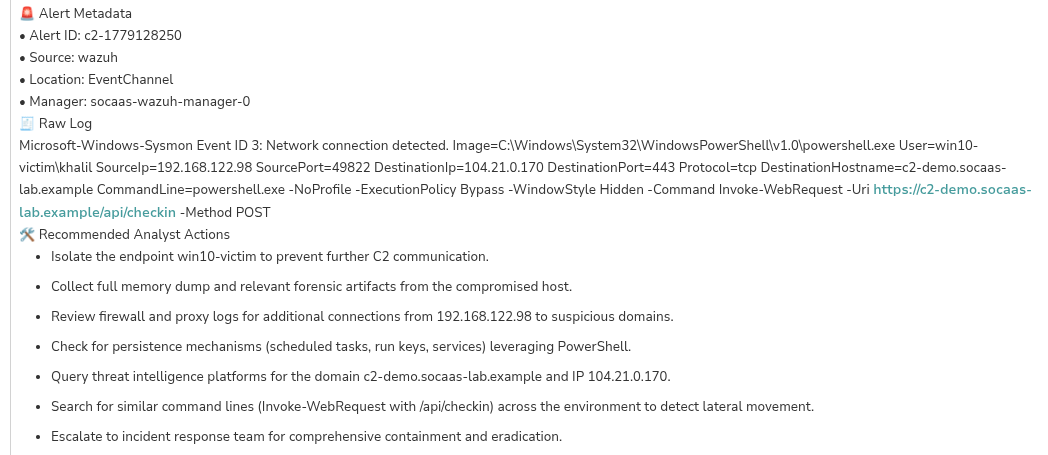
\includegraphics[width=0.95\textwidth]{figs/ai_recommendations_c2_beacon.png}
\caption{AI Recommended Analyst Actions for C2 Beacon Detection}
\label{fig:ch4-c2-ai-recommendations}
\end{figure}

The AI recommendation output identifies the suspicious outbound connection, highlights the endpoint and network destination context, and proposes containment and investigation actions. These recommendations support analyst triage but do not replace analyst validation.

Additional data exfiltration recommendation evidence is included in Chapter~4 because it directly supports the AI-assisted alert triage section.
